\documentclass[letterpaper]{article}
\usepackage[preprint]{aaai2027}
\usepackage{times}
\usepackage{helvet}
\usepackage{courier}
\usepackage[hyphens]{url}
\usepackage{graphicx}
\usepackage{amsmath,amssymb,booktabs}
\usepackage{natbib}
\urlstyle{rm}
\frenchspacing
\setcounter{secnumdepth}{0}
\pdfinfo{/Title (Normalization-Aware Readout for Targeted Memory Control in Hybrid Language Models) /Author (Lu-Yen Marco Tuan) /Subject (Working paper, November 14, 2026)}
\title{Normalization-Aware Readout for Targeted Memory Control\\in Hybrid Language Models}
\author{Lu-Yen Marco Tuan}
\affiliations{Department of Cognitive Science\\University of California San Diego\\Working paper --- November 14, 2026}
\newcommand{\R}{\mathbb{R}}
\begin{document}
\maketitle
\pagestyle{plain}
\thispagestyle{plain}

\begin{abstract}
We investigate why information encoded in the native memory of hybrid
language models can remain behaviorally inaccessible, and develop a
normalization-aware readout method that enables targeted memory updates to
influence model outputs. The method forecasts a specified write and
optimizes its read contrast after headwise normalization, jointly across
heads sharing a query. On independent synthetic retrieval cohorts, it
improves answer-control success from 45.9\% to 70.5\% in Qwen3.5-9B and
from 84.8\% to 100\% in Qwen3.5-27B while preserving all tested unaffected
answers. A simplified, native-initialized solver additionally reduces
total intervention time by 21.8\% relative to our four-start, 16-step
reference solver without sacrificing observed control success. These
results identify normalized readout geometry as a useful design target
for making specified runtime-memory updates behaviorally effective.
\end{abstract}

\section{Introduction}
An internal memory change need not change a language model's answer.
Even when a targeted write introduces a relevant state difference,
subsequent computation may fail to express that difference in the output.
This separates the presence of information in runtime memory from its
behavioral accessibility. A useful intervention must therefore address
both what is written and how the model reads it.

Hybrid language models offer a concrete setting for studying this
distinction. Recurrent linear-attention blocks compress history into
shared states, while full-attention blocks maintain token-indexed caches.
Prior work decomposes recurrent recall into writing, retention, and
access, and shows that full-attention caches can carry the values used
for recall in hybrid models \citep{lee2026}. Recurrent blocks can also
construct the address used by later attention readers, with more
distributed address computation at larger scales \citep{zeng2026}.
These findings motivate interventions on both a local value-bearing
state and a distributed address path.

Our central idea is to optimize the state change that survives the
model's normalization. A query that maximizes a raw memory response
can emphasize a change that normalization largely removes. The
background state determines this attenuation, and several value heads
share each query. We therefore forecast edited and unedited states,
evaluate their finite normalized read contrast jointly across shared
heads, and optimize that contrast within a fixed neighborhood of the
native query. Model weights remain fixed.

This working paper focuses on the controlled synthetic-retrieval
results. With fixed write and query budgets within each model, normalized
reading improves answer control on independent 9B and 27B cohorts.
The 27B study further shows that one native initialization preserves
the reference solver's target answers while reducing total measured
intervention time. The contribution is a write-conditioned readout
objective and its evaluated implementation for targeted runtime-state
interventions.

\section{Task and Controlled Interventions}
Each independent seed defines eight animal--letter assignments and paired
counterfactuals. We present the same instance in table and prose formats;
the two presentations remain grouped in the analysis. Prompts contain
84--127 tokens, including the fixed chat-template suffix. The endpoint
is the unrestricted full-vocabulary top output token immediately after
the suffix. Answer-control success means selecting the donor's intended
letter after the specified internal intervention.

For Qwen3.5-9B, the donor exchanges two assignments, changing the requested
value. The recipient retains its own prompt and receives the newest
convolution-value slot from layer 28, heads 28 and 29: 256 scalar
coordinates in total. A shared query can be changed at each of the final
four prompt positions. For Qwen3.5-27B, the dictionary stays fixed and
the donor asks about another key. A fixed write transfers nine
recurrent/convolution groups, totaling 465,408 coordinates. Queries can
change at four positions in four selected layers, giving 16 slots.
All layer and head indices are zero-based. The write precedes the four
suffix positions. Write sites and query locations were selected on
earlier development inputs and fixed before confirmation.

\begin{table}[t]
\centering
\small
\begin{tabular}{lrr}
\toprule
 & 9B & 27B\\
\midrule
Independent seeds & 256 & 128\\
Target presentations & 512 & 256\\
Written coordinates & 256 & 465,408\\
Available query slots & 4 & 16\\
Value heads per shared query & 2 & 3\\
Query dimension & 128 & 128\\
\bottomrule
\end{tabular}
\caption{Cohorts and budgets for the headline comparisons. The 27B cohort
is the final single-start confirmation. Methods share the write and
available query slots within each model; write paths differ across models.}
\label{tab:design}
\end{table}

Three paired preservation arms accompany each reader. A nuisance donor
changes unrelated assignments while preserving the queried binding.
Two further arms apply the target and nuisance readers to unwritten
recipient states. Their desired output is the recipient's original
answer. These arms distinguish useful control of a specified update
from indiscriminate answer changes. The tests provide explicit
counterfactual targets and preservation endpoints, following the
importance of corruption and measurement choices in activation
patching \citep{zhang2024}.

\section{Normalization-Aware Readout}
\subsection{Forecasting the State Difference}
For a Gated DeltaNet value head, write the recurrent state as
$S_t\in\R^{d_k\times d_v}$, with key $k_t$, value $v_t$, retention
$\alpha_t$, and update gate $\beta_t$. Its update is
\begin{equation}
S_t=\alpha_t S_{t-1}+\beta_t k_t
\bigl(v_t-\alpha_t S_{t-1}^{\top}k_t\bigr)^{\top}.
\end{equation}
This combines retention and delta-rule writing \citep{yang2025}.
In the 9B value-write setting, the paired trajectories share keys and
gates, so their difference satisfies
\begin{equation}
\Delta S_t=\alpha_t(I-\beta_t k_tk_t^{\top})\Delta S_{t-1}
+\beta_t k_t\Delta v_t^{\top}.
\label{eq:forecast}
\end{equation}
The convolution determines $\Delta v_t$. We propagate the write to
each permitted read position and check the forecast against execution.

The 27B write changes recurrent and convolution states at multiple
layers. At each read layer, two shadow recurrences begin from the
recipient and edited caches and consume the current branch's actual
incoming activations. Their difference represents the layer-local
initial write conditional on those activations. This conditioning
accounts for inputs already changed by earlier interventions; the
shadow matching the live branch is checked against the recurrent kernel.

Forecasting is used locally at the allowed intervention sites. It does
not require differentiating through the full language model or changing
the stored model parameters. At a read position, the solver receives
the paired forecast states and returns one replacement query; ordinary
downstream computation then determines the output token. Thus the
memory write supplies the intended change, while the reader controls
its expression through an existing computational path.

\subsection{Optimizing the Normalized Contrast}
Let $S_h$ and $S_h+\Delta S_h$ be the forecast states for value head $h$.
For a query $q$ in the kernel's effective coordinates, define
\begin{align}
N(x)&=\frac{x}{\sqrt{\|x\|_2^2/d_v+\epsilon}},\quad \epsilon=10^{-6},\\
D_h(q)&=N\bigl((S_h+\Delta S_h)^\top q\bigr)
-N\bigl(S_h^\top q\bigr).
\end{align}
Normalization is evaluated before the learned normalization weight
and output gate. If $q_0$ is the native query, let $T$ be the unit vector
formed by concatenating $D_h(q_0)$ across the heads sharing that query,
and let $T_h$ be its headwise components. We solve
\begin{align}
\max_q\quad &\sum_h\langle D_h(q),T_h\rangle,\label{eq:objective}\\
\text{subject to}\quad &\|q\|_2=\|q_0\|_2,\qquad
\cos(q,q_0)\geq 0.5.\nonumber
\end{align}
The direction $T$ comes from the specified write's native read contrast;
the objective uses internal states rather than an output-label loss.

The geometric motivation follows directly from the derivative of RMS
normalization. For $\rho=(\|x\|_2^2/d_v+\epsilon)^{1/2}$,
\begin{equation}
J_N(x)=\rho^{-1}I-\frac{xx^\top}{d_v\rho^3}.
\end{equation}
When $x\ne0$, a perturbation parallel to $x$ is scaled by
$\epsilon/\rho^3$, whereas an orthogonal perturbation is scaled by
$1/\rho$. Thus a large raw change aligned with the background read
can have little normalized effect. Equation~\ref{eq:objective} uses
the finite contrast to incorporate this geometry jointly across heads.

\paragraph{A shared query creates a joint readout problem.}
Optimizing a head in isolation can ignore how the same query changes
its neighboring value heads. We instead concatenate their native
contrasts to construct a single target direction and sum the headwise
alignment scores. The norm constraint preserves query magnitude, and
the angular cap restricts rotation to at most $60$ degrees from the
native direction. These restrictions make the intervention budget
explicit. They do not constrain later activations or force the desired
token: answer control remains an observed consequence of the modified
read and the model's remaining computation.

\subsection{Solvers and Comparisons}
The 9B reference optimizer uses four initial directions and 80 projected
gradient iterations, comparing seven candidate step sizes with the
current point at each iteration. Starts include the native direction,
a leading singular vector of the concatenated state changes, and two
whitened directions. The final 27B solver uses only the native direction
and 16 iterations. It retains the objective, step-size choices, angular
constraint, and native query norm. Each optimized query is shared across
its value heads and cast back to inference precision.

The primary 9B comparator is a whitened-key reader. It applies the
inverse regularized background covariance to the source-key direction,
using $C=\sum_hS_hS_h^\top$ and
$\lambda=\max(10^{-3}\operatorname{tr}(C)/128,10^{-12})$.
The primary 27B baselines are raw SVD, which uses a leading left singular
vector of the concatenated $\Delta S_h$, and a shared direction fitted
on four development seeds. Simple directions are oriented toward the
native query and norm-matched. They receive the same write and available
query slots. The headline comparisons retain the stronger original
simple directions without imposing the optimizer's angular cap.

\begin{figure*}[t]
\centering
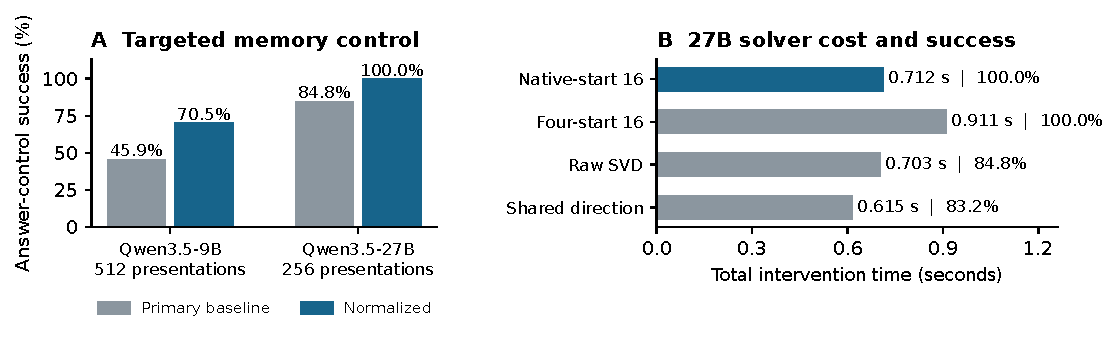
\includegraphics[width=\textwidth]{../figures/control_and_cost.pdf}
\caption{Independent confirmation of answer control and solver efficiency.
Left: each model's primary baseline versus normalized reading; counts
include both formats of every seed. Right: the same 27B cohort compares
total intervention time across readers. Both normalized solvers control
256/256 targets; the native-start solver reduces time by 21.8\% relative
to the four-start, 16-step reference. All displayed readers preserve
every answer in the three paired control arms.}
\label{fig:results}
\end{figure*}

\section{Independent Confirmation Results}
Methods, input generation, exclusions, and analyzers were fixed before
collecting each confirmation cohort. Seed identifiers and tokenized
target prompts were checked against earlier inputs. The independent
unit is a seed: we average its two formats and bootstrap paired
differences over seeds with 20,000 replicates. The 9B primary comparison
uses a 95\% interval; the two 27B primary comparisons each use a 97.5\%
interval to adjust for their joint test. Table~\ref{tab:design} describes
the two cohorts supporting the abstract.

\paragraph{Local value updates become behaviorally effective at 9B.}
Normalized reading controls 361/512 target presentations (70.51\%),
compared with 235/512 (45.90\%) for whitened key. The paired gain is
24.61 percentage points, with a 95\% interval of [20.51, 28.71]. Table
format improves from 124/256 to 167/256, and prose from 111/256 to
194/256. There are 128 presentation-level wins and two losses.
The same memory write under the native query controls 0/512 targets,
making the distinction between a state update and its behavioral use
particularly clear.

The advantage also holds over whitened SVD (232/512) and an
output-aware normalized variant (330/512). Temporal placement matters:
using all four permitted read positions controls 361/512 answers,
versus 82/512 using only the final position, a gain of 54.49 points
[49.22, 59.96]. This timing comparison spends four query slots instead
of one; the primary reader comparison keeps all four slots available
to both methods.

\paragraph{Distributed address updates show the same benefit at 27B.}
On 128 new seeds, the native-start, 16-step reader controls all 256
target presentations. Raw SVD controls 217/256 (84.77\%) and minimal
shared reading controls 213/256 (83.20\%). The paired gains are 15.23
points [9.38, 21.88] and 16.80 points [10.94, 23.44], respectively,
using the adjusted intervals. These comparisons improve on 27 and 32
seeds, respectively, and lose on none. Figure~\ref{fig:results} shows
the primary control and cost comparisons.

\paragraph{All tested unaffected answers are preserved.}
Normalized reading retains 512/512 answers in each of the three 9B
preservation arms and 256/256 in each 27B arm. Thus the selected reader
preserves 1,536 evaluated control presentations at 9B and 768 at 27B.
The primary baselines also preserve these answers. Preservation refers
to the tested nuisance and unwritten conditions, with formats grouped
by seed; it is not an estimate over arbitrary unrelated prompts.

\paragraph{The paired design separates format variation from replication.}
The 512 target presentations at 9B represent 256 independent dictionaries,
and the 256 presentations at 27B represent 128. Resampling complete seed
groups retains the dependence between table and prose renderings and
between the readers evaluated on each input. The positive intervals
therefore reflect paired gains on new seed groups, rather than treating
multiple renderings as additional independent experiments. All target
presentations contribute to the reported rates, including cases where
the desired answer was not obtained.

\section{A Simpler Solver at Lower Cost}
The final 27B confirmation compares the native-start solver directly
with the four-start, 16-step batched reference on the same cases.
Both control 256/256 target answers. Mean total intervention time falls
from 0.9108 to 0.7120 seconds, a 21.83\% reduction. The paired
seed-bootstrap time ratio is 0.7817, with a 95\% interval of
[0.7808, 0.7827]. No seed loses a reference-controlled answer; the
one-sided 95\% upper bound on the seed-loss probability is 2.31\%.
Preservation is measured at the answer endpoint, without requiring
identical intermediate queries or logits.

The native start removes SVD, whitening, and alternative-start
construction while retaining the normalized objective. The observed
cost is close to raw SVD's 0.7027 seconds, with 15.23 percentage points
more answer control. Minimal shared reading takes 0.6149 seconds.
These comparisons expose the measured accuracy--cost tradeoff without
assuming that the normalized reader is the cheapest intervention.

Timing includes both recipient and donor prefills, state cloning and
writing, and synchronized continuation with query design, transfers,
and controller work. Scoring, cache hashing, and trace export occur
after the timer. Method order rotates across cases. Minimal shared
reading omits unused forecasts and diagnostics; it matches the
instrumented shared implementation's full logits, cache digests, and
query arrays on all 1,024 branches. The 27B timings were collected on
an NVIDIA RTX PRO 6000 Blackwell Workstation Edition with BF16
inference, PyTorch 2.9.0, and Transformers 5.22.1. The 9B confirmation
used NVIDIA GB10 and BF16 inference. Costs are within-cohort measurements.

\section{Relation to Prior Work}
\paragraph{Memory mechanisms.}
The write--retain--access account of \citet{lee2026} supplies a useful
decomposition of recurrent memory. The address-building mechanism of
\citet{zeng2026} explains how recurrent computation can influence
retrieval even when full attention supplies the recalled value. Our
experiments use these distinct roles to define concrete intervention
paths. The added question is constructive: given a fixed state write,
which allowed query makes that write more likely to control the answer?

\paragraph{Architecture and intervention.}
Gated DeltaNet combines retention with delta-rule updates
\citep{yang2025}. Our state forecast follows that recurrence, while
the normalized objective uses the pretrained model's existing readout.
The method acts at inference time on runtime states and queries. It
does not retrain the recurrent update or introduce a learned external
memory. This setting makes the computational effect of the reader
directly comparable across the same specified writes.
Muir addresses state-row norm imbalance with a trained matched-filter
read gate and architectural changes \citep{gangavarapu2026}. Our reader
instead optimizes a specified write's finite normalized contrast within
a fixed pretrained model.

\paragraph{Behavioral evidence.}
Activation-patching conclusions depend on intervention construction
and the endpoint used to measure its effect \citep{zhang2024}.
Here the donor specifies the counterfactual answer, unrestricted
top-token selection measures behavioral control, and paired nuisance
and unwritten branches test answer preservation. The read objective
is a mechanistic surrogate; its value is established by these output
comparisons rather than by objective improvement alone.

\section{Discussion and Conclusion}
The results support a concrete mechanism for improving targeted memory
control: optimize the contrast that remains after normalization, taking
the background state and shared-query structure into account. The
controlled intervention makes this operational. A specified write
provides the target state difference, a forecast identifies subsequent
read opportunities, and a constrained query makes that difference
more effective at the answer endpoint.

The value and address experiments use different fixed write paths in
two sizes of the Qwen3.5 family. They establish the utility of a common
readout objective within those budgets, rather than a cross-model
scaling law. The evidence concerns short synthetic dictionaries with
explicit donors and single-token answers. Applying the method to
natural document updates requires specifying the intended write and
evaluating task utility in that setting. Within the evaluated scope,
normalized reading raises answer control while preserving every
tested unaffected answer, and a single native initialization makes
the 27B intervention faster without loss of observed control success.

\paragraph{Evidence and reproducibility.}
The accompanying artifact records the source repository revision,
complete score rows for the two headline cohorts, the original
aggregate analyses, and an independent script that recomputes the
reported paired effects and timing ratio. The paper and vector figure
can be rebuilt without model inference. The archived results are
reused here to give a focused account of controlled memory readout;
no new model experiment is claimed by this working-paper extraction.

\begin{thebibliography}{5}
\bibitem[Gangavarapu et~al.(2026)]{gangavarapu2026}
Gangavarapu, T.; Tabak, G.; and Schaefer, C.~J.~S. 2026.
Muir: Linear Attention with Sensitivity-Allocated Gating and Matched-Filter
Readout. \emph{arXiv:2611.08376}.
\url{https://arxiv.org/abs/2611.08376}.

\bibitem[Lee et~al.(2026)]{lee2026}
Lee, K.; Park, J.; Kim, S.; and Ko, J. 2026.
How Linear Attention Remembers. \emph{arXiv:2609.33093}.
\url{https://arxiv.org/abs/2609.33093}.

\bibitem[Yang et~al.(2025)]{yang2025}
Yang, S.; Kautz, J.; and Hatamizadeh, A. 2025.
Gated Delta Networks: Improving Mamba2 with Delta Rule.
In \emph{International Conference on Learning Representations}.
\url{https://arxiv.org/abs/2412.06464}.

\bibitem[Zeng et~al.(2026)]{zeng2026}
Zeng, W.; Feng, C.; and Chen, Y. 2026.
Who Asks, Who Answers: Linear Attention Builds the Query in Hybrid
Language Models. \emph{arXiv:2611.01909}.
\url{https://arxiv.org/abs/2611.01909}.

\bibitem[Zhang and Nanda(2024)]{zhang2024}
Zhang, F.; and Nanda, N. 2024.
Towards Best Practices of Activation Patching in Language Models:
Metrics and Methods. In \emph{International Conference on Learning
Representations}. \url{https://arxiv.org/abs/2309.16042}.
\end{thebibliography}
\end{document}
